% Figure 6(a): The finite-matching numerical pipeline implemented in the
% companion repository.
% Authors: Dr. Davide Batic and Dr. Denys Dutykh
%          (Mathematics Department, Khalifa University of Science and
%           Technology, Abu Dhabi, UAE)
\documentclass[tikz,border=6pt]{standalone}
% ============================================================================
% Shared TikZ style for the figures of the Kerr–Dirac two-channel scattering
% manuscript (compiled standalone into ../latex/figures/).
% Authors: Dr. Davide Batic and Dr. Denys Dutykh
%          (Mathematics Department, Khalifa University of Science and
%           Technology, Abu Dhabi, UAE)
%
% Visual language (used consistently across all figures):
%   * horizon channel      : navy  (chH)
%   * spatial-infinity     : teal  (chI)
%   * accents / emphasis   : gold  (acc)
%   * future/out data      : solid arrows
%   * past/in data         : dashed arrows
%   * proved here          : solid box border
%   * imported input       : light-gray filled box
%   * conditional          : dashed box border
% ============================================================================
\usepackage{amsmath,amssymb}
\usetikzlibrary{arrows.meta,positioning,decorations.pathmorphing,calc,matrix}

\definecolor{chH}{HTML}{142D6E}   % horizon channel (navy)
\definecolor{chI}{HTML}{0E6E6E}   % spatial-infinity channel (teal)
\definecolor{acc}{HTML}{9A7A2E}   % gold accent
\definecolor{warm}{HTML}{9C5310}  % sienna (warnings/exclusions)
\definecolor{ltg}{HTML}{F2F2F2}   % light gray fill (imported)

\tikzset{
  outarr/.style={-{Stealth[length=2.6mm]}, line width=0.9pt},
  inarr/.style={-{Stealth[length=2.6mm]}, line width=0.9pt, dashed},
  axis/.style={-{Stealth[length=2.2mm]}, line width=0.6pt, gray!70!black},
  wavyH/.style={chH, decorate, decoration={snake, amplitude=0.45mm, segment length=2.6mm}},
  wavyI/.style={chI, decorate, decoration={snake, amplitude=0.45mm, segment length=2.6mm}},
  proved/.style={draw, line width=0.7pt, rounded corners=2pt, inner sep=4pt},
  imported/.style={draw=gray!60, fill=ltg, line width=0.5pt, rounded corners=2pt, inner sep=4pt},
  conditional/.style={draw, dashed, line width=0.7pt, rounded corners=2pt, inner sep=4pt},
  lab/.style={font=\small},
  slab/.style={font=\footnotesize},
  tlab/.style={font=\scriptsize},
}

\begin{document}
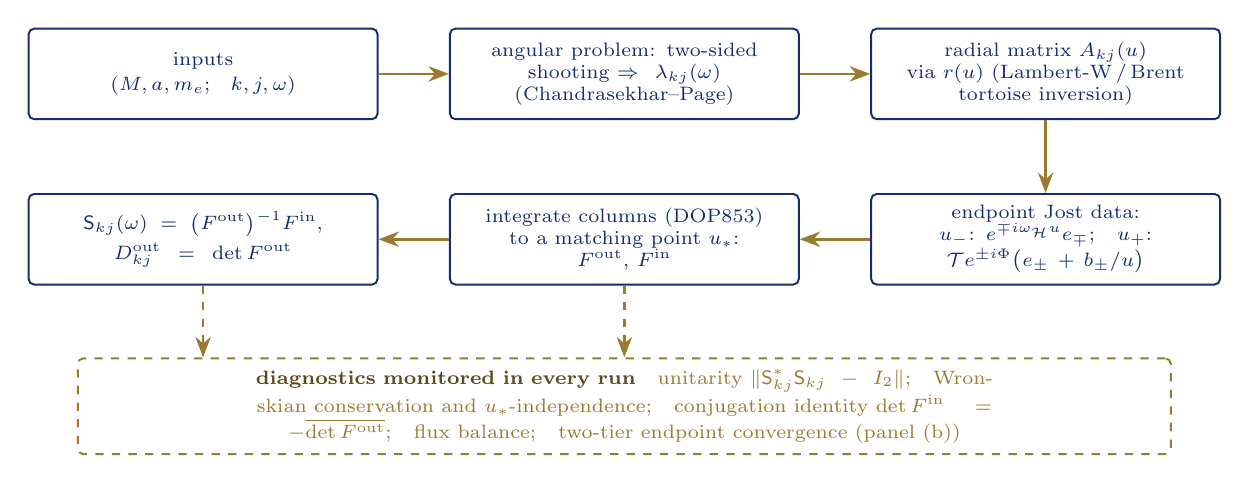
\begin{tikzpicture}[x=1cm,y=1cm,
  stage/.style={proved, chH, tlab, align=center, text width=4.15cm, minimum height=1.15cm},
  flow/.style={outarr, acc}]

% ---- row 1 -----------------------------------------------------------------
\node[stage] (in)  at (0.0,0)  {inputs\\[0.4mm] $(M,a,m_e;\;k,j,\omega)$};
\node[stage] (ang) at (5.35,0) {angular problem: two-sided\\ shooting $\Rightarrow\lambda_{kj}(\omega)$\\ (Chandrasekhar--Page)};
\node[stage] (rad) at (10.7,0) {radial matrix $A_{kj}(u)$\\ via $r(u)$ (Lambert-W\,/\,Brent\\ tortoise inversion)};
% ---- row 2 -----------------------------------------------------------------
\node[stage] (S)   at (0.0,-2.1)  {$\mathsf S_{kj}(\omega)=\bigl(F^{\rm out}\bigr)^{-1}F^{\rm in}$,\\[0.4mm] $D^{\rm out}_{kj}=\det F^{\rm out}$};
\node[stage] (ode) at (5.35,-2.1) {integrate columns (DOP853)\\ to a matching point $u_*$:\\ $F^{\rm out},\,F^{\rm in}$};
\node[stage] (jost) at (10.7,-2.1) {endpoint Jost data:\\ $u_-$: $e^{\mp i\omega_{\mathcal H}u}e_\mp$;\quad $u_+$:\\ $\mathcal Te^{\pm i\Phi}\bigl(e_\pm+b_\pm/u\bigr)$};
% ---- flow ------------------------------------------------------------------
\draw[flow] (in) -- (ang);
\draw[flow] (ang) -- (rad);
\draw[flow] (rad) -- (jost);
\draw[flow] (jost) -- (ode);
\draw[flow] (ode) -- (S);
% ---- diagnostics -----------------------------------------------------------
\node[conditional, acc, tlab, align=center, text width=13.6cm, anchor=north]
  (diag) at (5.35,-3.6)
  {\textcolor{acc!60!black}{\textbf{diagnostics monitored in every run}}\quad
   unitarity $\|\mathsf S_{kj}^*\mathsf S_{kj}-I_2\|$;\quad
   Wronskian conservation and $u_*$-independence;\quad
   conjugation identity $\det F^{\rm in}=-\overline{\det F^{\rm out}}$;\quad
   flux balance;\quad two-tier endpoint convergence (panel (b))};
\draw[inarr, acc] (S.south) -- (S.south |- diag.north);
\draw[inarr, acc] (ode.south) -- (ode.south |- diag.north);

\end{tikzpicture}
\end{document}
